% https://texnique.fr/osqa/questions/6660/tikz-alignement-de-nodes/6663
\documentclass{beamer}
\usepackage{tikz}
\begin{document}
\begin{frame}
\frametitle{Occupation du site de Bibracte}
\centering
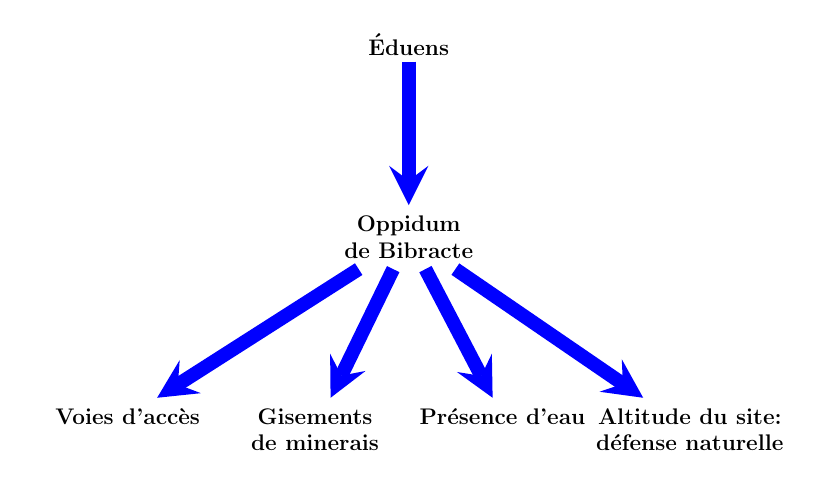
\begin{tikzpicture}[
        scale=.68,
        every node/.style={scale=.68,text width=3.5cm,text centered,anchor=north,font=\large\bfseries,color=black},
        level/.style={sibling distance=3.5cm,level distance=3cm,-stealth,line width=5pt,blue},  
]
  \node {Éduens}
    child {node {Oppidum de Bibracte}
      child {node {Voies d'accès}}
      child {node {Gisements de minerais}}
      child {node {Présence d'eau}}
      child {node {Altitude du site: défense naturelle}}            
    };
\end{tikzpicture}

\end{frame}
\end{document}